\documentclass[a4paper,11pt]{article}
\newlength{\outerbordwidth}
\pagestyle{empty}
\raggedbottom
\raggedright
\usepackage[svgnames]{xcolor}
\usepackage{framed}
\usepackage{times}
\usepackage{tabu}
\usepackage{tocloft}
\usepackage{graphicx}
\usepackage{multirow}
\usepackage[utf8]{inputenc}
\usepackage{tabularx}
\title{Saim-CV}

%-----------------------------------------------------------
%Edit these values as you see fit

\setlength{\outerbordwidth}{3pt}  % Width of border outside of title bars
\definecolor{shadecolor}{gray}{0.2}  % Outer background color of title bars (0 = black, 1 = white)
\definecolor{shadecolorB}{gray}{1}  % Inner background color of title bars


%-----------------------------------------------------------
%Margin setup

\setlength{\evensidemargin}{-0.25in}
\setlength{\headheight}{0in}
\setlength{\headsep}{0in}
\setlength{\oddsidemargin}{-0.25in}
\setlength{\paperheight}{11in}
\setlength{\paperwidth}{8.5in}
\setlength{\tabcolsep}{0in}
\setlength{\textheight}{9.5in}
\setlength{\textwidth}{7in}
\setlength{\topmargin}{-0.3in}
\setlength{\topskip}{0in}
\setlength{\voffset}{0.1in}

\newcommand{\resitem}[1]{\item #1 \vspace{-2pt}}
\newcommand{\resheading}[1]{\vspace{8pt}
    \parbox{\textwidth}{\setlength{\FrameSep}{\outerbordwidth}
        \begin{shaded}
            \setlength{\fboxsep}{0pt}\framebox[\textwidth][l]{\setlength{\fboxsep}{4pt}\fcolorbox{shadecolorB}{shadecolorB}{\textbf{\sffamily{\mbox{~}\makebox[6.762in][l]{\large #1} \vphantom{p\^{E}}}}}}
        \end{shaded}
    }\vspace{-5pt}
}
\newcommand{\ressubheading}[4]{

    \begin{tabular*}{6.5in}{l@{\cftdotfill{\cftsecdotsep}\extracolsep{\fill}}r}
        \textbf{#1} & #2 \\
        \textit{#3} & \textit{#4} \\
    \end{tabular*}\vspace{-6pt}}
%-----------------------------------------------------------


\begin{document}
    
    %-----------------------------------------------------------
    %Insert profile photo 
    \begin{tabular*}{7in}{l@{\extracolsep{\fill}}r}
        & \multirow{1}{*}{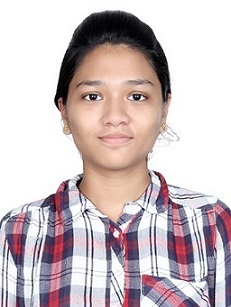
\includegraphics[scale=0.025]{Profile}}\\
         \\
        %-----------------------------------------------------------  
        \textbf{\Large Saim Shaikh } & \\
        Fr. Conceicao Rodrigues College of Engineering, Bandra  \\
        Email: saimshaikh8297@gmail.com \\
        Contact: 8286515545\\
    \end{tabular*}

  %%%%%%%%%%%%%%%%%%%%%%%%%%%%%%
    \resheading{Objective}
    %%%%%%%%%%%%%%%%%%%%%%%%%%%%%%
    \begin{itemize}
        \item
            To practically apply my knowledge while working on projects as well as to learn new things along the way 
    \end{itemize}
    %%%%%%%%%%%%%%%%%%%%%%%%%%%%
 \resheading{Education}

\begin{tabu} to 1\textwidth { | X[c] | X[c] | X[c] | X[c]| X[c]|}
 \hline
 {\bf Degree} & {\bf College /School} & {\bf University} & {\bf Year of Passing} & {\bf Score}\\
 \hline
 BE. Info Tech. & Fr.CRCE &Mumbai University & 2019 & 7.3 (Till Sem V) \\
\hline
HSC & Shri T.P. Bhatia College (Mumbai)& MSBSHSE(State Board) & 2015 & 75\\
\hline
SSC & Holy Cross Convent School (Mira Road) & MSBSHSE(State Board) & 2013 & 89.82\\
\hline
\end{tabu}

\resheading{Projects}
    %%%%%%%%%%%%%%%%%%%%%%%%%%%%%%
\begin{itemize}
      \item
        \ressubheading{Automated Traffic Surveillance System}{}{eYIC-2018}{}
        \begin{itemize}
            \resitem{Involves 3 Modules Signal Offenders,Speed Detection,Helmet Detection}
            \resitem{Individually implemented Vehicle Detection and Helmet Detection using FRCNN algorithm}
            \resitem{Implemented using Tflearn,Tensorflow,OpenCV}
        \end{itemize}
\end{itemize}
    %%%%%%%%%%%%%%%%%%%%%%%%%%%%%%

  \resheading{Training}
    %%%%%%%%%%%%%%%%%%%%%%%%%%%%%%
    \begin{itemize}
        \resitem {{\bf Machine learning} from \textit {"Coursera"} by Andrew Ng.(Audited)}
        \resitem{{\bf Programming for Everybody (Getting Started with Python)}\textit{ Michigan State University}{ on Coursera}}
        \resitem{{\bf Practical Deep Learning for Coders using PyTorch}\textit{ Fast.ai}}
    \end{itemize}

  %%%%%%%%%%%%%%%%%%%%%%%%%%%%%%
    \resheading{Technical Skills}
 \begin{itemize}
        \resitem{{\bf Programing Languages:} Python, Java , SQL also familiar with C/C++ and Octave}
        \resitem{{\bf Frameworks and Libraries:} NumPy,MatplotLib,Tensorflow,TFLearn,PyTorch,OpenCV}
        \resitem{{\bf Software:} Adobe Photoshop, Android Studio}
    \end{itemize}

 \resheading{Soft Skills}
    %%%%%%%%%%%%%%%%%%%%%%%%%%%%%%
    \begin{itemize}
       \resitem{Leadership}
        \resitem{Like to work as a Team}
        \resitem{Decisive}
        \resitem{Strong work Ethic and Punctuality}
        \resitem{Problem Solving}
        \resitem{Ability to Work Under Pressure}
    \end{itemize}

 \resheading{Co-Curricular Activity}
    %%%%%%%%%%%%%%%%%%%%%%%%%%%%%%
    \begin{itemize}
        \resitem{Won the {\bf"Best Algorithm Design"} award at eYIC-2018}
        \resitem{Participated in State Level Project Presentation Competition Held at Fr.CRCE Bandra}
        \resitem{Participated in State level hackthon ERR404}
    \end{itemize}
   
 \resheading{Extra-Curricular Activity}
    %%%%%%%%%%%%%%%%%%%%%%%%%%%%%%
    \begin{itemize}
       \resitem{Senior Council member and {\bf PR and Marketing Head} at IEEE-CRCE}
    \end{itemize}

 %%%%%%%%%%%%%%%%%%%%%%%%%%%%%%
    \resheading{Personal Details}
    %%%%%%%%%%%%%%%%%%%%%%%%%%%%%%
    \begin{itemize}
        \resitem{{\bf Father's Name:} Sajid A. Shaikh}
        \resitem{{\bf Mother's Name:} Saniya S. Shaikh}
        \resitem{{\bf Sex:} Male}
        \resitem{{\bf Date of Birth:} 8\textsuperscript{th} February 1997}
        \resitem{{\bf Nationality:} Indian}
        \resitem{{\bf Marital Status:} UnMarried}
    \end{itemize}
   
 \resheading{Declaration}
    %%%%%%%%%%%%%%%%%%%%%%%%%%%%%%
    \begin{itemize}
        \item
        All the information mentioned in the resume is correct to the best of my knowledge and belief.
    \end{itemize}
 
\end{document}



